\documentclass[11pt]{article}

\usepackage[final]{nips}
%\usepackage{times}
\usepackage{alltt}
\usepackage{graphicx}
\usepackage{hyperref}

%
\usepackage[utf8x]{inputenc}
\usepackage[labelformat=simple]{subcaption}
\usepackage{paralist}
\usepackage{listings}
\usepackage[dvipsnames]{xcolor}
\usepackage{siunitx}
\usepackage{comment}
\usepackage{enumitem}
\usepackage{booktabs}
\usepackage{algorithm}
\usepackage[noend]{algpseudocode}

\usepackage{fancyvrb}
\VerbatimFootnotes
\usepackage{multicol}
\usepackage{multirow}
\usepackage{bold-extra}
\usepackage{pgfplots}

\setcitestyle{numbers,square,comma}

% Centered fixed width table cell
\newcolumntype{x}[1]{>{\centering\let\newline\\\arraybackslash\hspace{0pt}}p{#1}}

\renewcommand\thesubfigure{(\alph{subfigure})}

\setlength{\pltopsep}{5pt}
\setlength{\footskip}{30pt}
\setlength{\baselineskip}{1.3\baselineskip}
\renewcommand\arraystretch{1.2}

\definecolor{grey}{rgb}{0.3,0.3,0.3}
\definecolor{darkgreen}{rgb}{0,0.3,0}
\definecolor{darkblue}{rgb}{0,0,0.3}
\definecolor{lightgrey}{rgb}{0.9,0.9,0.9}
\definecolor{darkgrey}{rgb}{0.1,0.1,0.1}
%\renewcommand{\ttdefault}{pcr}
\lstset{%
% indexing
    numbers=none,
    numberstyle=\small,%
% character display
    showstringspaces=false,
    showspaces=false,%
    tabsize=4,%
    columns=fullflexible,
    extendedchars=false,
% style
    frame=none,%
    basicstyle=\tt,%
    keywordstyle=\color[rgb]{0,0.2,0.6},%
    stringstyle=\color[rgb]{0,0.5,0},%
    commentstyle=\color{grey}\itshape,%
    identifierstyle=,%
    breaklines=true,                % sets automatic line breaking
    escapeinside={/*@}{@*/},
    keepspaces=true,
    columns=fixed,basewidth=.52em,
}

\lstdefinelanguage
   [x64]{Assembler}     % add a "x64" dialect of Assembler
   [x86masm]{Assembler} % based on the "x86masm" dialect
   % with these extra keywords:
   {morekeywords={vmulss,vaddss,vucomiss,addl,cmpl,vsubss},%
    morecomment=[l]{\#}} % etc.

\lstdefinelanguage
   [json]{EBNF} %
   [11]{C++} %
   {morekeywords={json,value,string,number,object,array,object-elements,array-elements,character,digit,digit-1-9,number,unicode},%
   alsoletter={-},%
   keywordstyle=\color[rgb]{0,0.2,0.6},%
   stringstyle=\color[rgb]{0,0.5,0},%
   deletestring=[b]{"},%
   string=[b]{'},%
   morestring=[d]{"}%
}

\setlist[itemize,1]{leftmargin=1.5em}
\setlist[enumerate,1]{leftmargin=1.5em}


%% Page layout
% \oddsidemargin 0pt
% \evensidemargin 0pt
% \textheight 600pt
% \textwidth 469pt
% \setlength{\parindent}{0em}
% \setlength{\parskip}{1ex}
% \usepackage[margin=1in,bottom=1in,top=1in]{geometry}


\begin{document}

\title{15-418/618 Project Report \\
MercuryJson: \\
Multi-Threaded JSON Parsing with SIMD
}

\author{
	Zecong Hu \\
	Carnegie Mellon University \\
	{\tt zeconghu@andrew.cmu.edu} \\
	\And
	Da Yin \\
	Carnegie Mellon University \\
	{\tt dayin@andrew.cmu.edu}
}
\date{}

\maketitle

\section{Summary}
We have implemented a parallel JSON parser with SIMD and multi-threading. Our implementation using 4 threads achieves on average $1.29\times$ speedup on large documents compared to a very strong baseline, and achieves comparable performance on small documents.


\section{Background}

\subsection{JSON Format}

JSON (JavaScript Object Notation)~\cite{bray2017javascript, crockford2006application} is a lightweight data-interchange format based on a subset of the JavaScript Programming Language, Standard ECMA-262 3rd Edition - December 1999. 

The EBNF~(Extended Backus-Naur form) of JSON grammar is described in figure~\ref{fig:ebnf-json}. JSON is built on two structures, namely objects and arrays. Objects are collections of key--value pairs and arrays are ordered lists of values. Keys are defined as strings composed of a sequence of zero or more Unicode characters, wrapped in double quotes, using backslash escapes. Values could be strings, numbers (integer or floating-point), keywords (\texttt{true}, \texttt{false}, \texttt{null}), or objects or arrays as described above.

\suppressfloats  % prevent the figure from popping up on top of first page

\begin{figure}
\lstset{language=[json]EBNF}
\begin{lstlisting}[basicstyle=\fontsize{8}{9}\tt,breaklines,numbers=none]
json            = value

value           = string | number | object | array | "true" | "false" | "null"

object          = "{" , object-elements, "}"
object-elements = string, ":", value, [ ",", object-elements ]

array           = "[", array-elements, "]"
array-elements  = value, [ ",", array-elements ]

string          = '"', { character }, '"'
character       = "\", ( '"' | "\" | "/" | "b" | "f" | "n" | "r" | "t" | "u", digit, digit, digit, digit ) | unicode

digit           = "0" | digit-1-9
digit-1-9       = "1" | "2" | "3" | "4" | "5" | "6" | "7" | "8" | "9"
number          = [ "-" ], ( "0" | digit-1-9, { digit } ), [ ".", { digit } ], [ ( "e" | "E" ), ( "+" | "-" ), { digit } ]
\end{lstlisting}
\caption{Extended Backus-Naur form of JSON grammar. The term ``\texttt{unicode}'' is defined as any Unicode character except those that must be escaped. Please refer to the JSON standards for details.}
\label{fig:ebnf-json}
\end{figure}

\subsection{JSON Parsing}

There are many existing JSON parsers used in various programming languages, most of which are based on finite state machines~(FSM). The state-of-the-art parser so far is \textit{simdjson} which utilizes SIMD instructions to accelerate the parsing process.

\textit{simdjson}~\cite{langdale2019parsing} divides the traditional FSM-based parsing into two stages. This two-stage method was first proposed in \textit{Mison}~\cite{li2017mison}, a fast JSON parser by Microsoft, based on structure speculation.
\textit{Mison} uses large datasets to learn to predict structural character positions which greatly eliminates branch prediction. While they can achieve over \SI{2}{GB/s} parsing speed as well, the speed across different datasets varies.

In \textit{simdjson}, by elegantly devising vector operations and using loop-unrolling tricks to avoid frequent branch predictions, it can reach over \SI{2}{GB/s} by exploiting parallelism in first stage which is independent of datasets. The first stage includes finding structural characters such as brackets and commas after picking out escape backslash characters and identifying literal values. Then, the parser will calculate the offsets between structural characters for use in second stage. Although the second stage for both \textit{Mison} and \textit{simdjson} are sequential, the usage of offset between structural characters greatly benefits parsing speed as it allows skipping over most content characters. \textit{simdjson} also utilizes a tape-based storage for fast creation of JSON structures, at the cost of slow random access.

Our work is mainly based on \textit{simdjson}. We also base our parser on the two-stage parsing procedure, and introduce multi-threading to further accelerate the second stage.

\subsection{General Parsing Algorithms}
\label{sec:parse-algo}

Our work is a small piece in the broad field of parsing. Although very different in implementation, our methods are in essence extensions built upon the fundamental parsing algorithms, namely \textbf{recursive descent} and  \textbf{shift-reduce}.

\textbf{Recursive descent} parsers are top-down parsers built from a set of mutually recursive procedures (or a non-recursive equivalent) where each such procedure implements one of the nonterminals of the grammar~\cite{burge1975recursive}. Recursive descent starts with the start symbol, and recursively expands each nonterminal symbol using production rules. Non-backtracking recursive descent parsers support LL($k$) grammars, which is a subset of unambiguous context-free grammars.

\textbf{Shift-reduce} parsers, on the other hand, are bottom-up parsers that incrementally builds the parse tree from bottom up. Shift-reduce parsers scan text from left to right, applying shift steps and reduces steps alternatively. A shift step consumes an input token, creates a single-node parse tree, and pushes it onto the parse stack. A reduce step applies a production rule to several parse trees off the stack top, replacing them with a joined tree with a new root symbol. Shift-reduce parsers support LR($k$) grammars, also a subset of unambiguous context-free grammars.

The JSON grammar is classified as both LL(1) and LR(1), thus both parsing algorithms are applicable to parsing JSON.

\section{Approach}

As mentioned, our approach uses a two-stage framework similar to that of \textit{simdjson}. Before introducing these two stages, we first define \textbf{structural characters} as the set of all square and curly brackets, colons, commas, and the first character of literal values (always quotes (\texttt{"})), numerical values (minus sign (\texttt{-}) or digits \texttt{0} through \texttt{9}), and keyword values (\texttt{t} for \texttt{true}, \texttt{f} for \texttt{false}, \texttt{n} for \texttt{null}). Among these characters, brackets, colons, and commas describe the JSON structure, while others indicate the beginning of a JSON value. If the document is valid, then structural characters along are sufficient to define the JSON structure, allowing us to skip over most characters in the second stage.

\subsection{Finding Structural Characters}

The first stage of parsing is to find the positions of structural characters. We reimplemented SIMD parsing algorithm in \textit{simdjson}. The original input is divided into groups size of $V$, where $V$ is the maximum data width that the processor supports divided by 8 (each character takes 8 bits). This could be 128, 256, or 512 bits depending on processor architecture. In our experiments, we use 256-bit AVX2 as default and 128-bit as fallback.

For each group of $V=32$ continuous characters in original input, we extract the position of structural characters inside into a separate indices array through the following steps:
\begin{enumerate}
    \item Compute the escape mask. Backslash characters~(\verb|\|) escape their following characters, and the aim of this step is to find out which characters need to be escaped. Continuous backslashes makes this computation a bit complicated. The process is shown as below. Note that our implementation is a little different from \textit{simdjson} --- while \textit{simdjson} only extracts ending escape positions, we extract all positions for later use.
\begin{lstlisting}[
    basicstyle=\fontsize{8}{9}\tt,
    language=C]
{ "\\\"Nam[{": [ 116,"\\\\" , 234, "true", false ], "t":"\\\"" }: input
___111________________1111_______________________________111____: B (Backslashes)
1_1_1_1_1_1_1_1_1_1_1_1_1_1_1_1_1_1_1_1_1_1_1_1_1_1_1_1_1_1_1_1_: E (Even idx mask)
_1_1_1_1_1_1_1_1_1_1_1_1_1_1_1_1_1_1_1_1_1_1_1_1_1_1_1_1_1_1_1_1: O (Odd idx mask)
// identify starting backslashes characters: those not preceded by backslashes
___1__________________1__________________________________1______: S = B & ~(B << 1)
// separate masks for starting backslashes located at odd and even indices
______________________1_________________________________________: ES = S & E
___1_____________________________________________________1______: OS = S & O
// compute carries by adding each mask with backslash sequences
___111____________________1______________________________111____: EC = B + ES
______1_______________1111__________________________________1___: OC = B + OS
// keep only odd-lengthed sequences by removing sequences that are not carried
______________________11111_____________________________________: ECE = EC ^ B
___1111__________________________________________________1111___: OCE = OC ^ B
// select odd offsets for even starts and even offsets for odd starts
_______________________1_1______________________________________: OD1 = ECE & O
____1_1___________________________________________________1_1___: OD2 = OCE & E
// merge results to obtain the escape mask
____1_1________________1_1________________________________1_1___: OD = OD1 | OD2
\end{lstlisting}
    \item Compute the literal mask which indicates which positions are inside a literal (string) value. By finding unescaped quotes and using carry-less multiplication \texttt{clmul}, we can compute the literal mask in only several cycles.
\begin{lstlisting}[
    basicstyle=\fontsize{8}{9}\tt,
    language=C]
{ "\\\"Nam[{": [ 116,"\\\\" , 234, "true", false ], "t":"\\\"" }: input
__1___1_____1________1____1________1____1___________1_1_1___11__: Q (Quotes)
______1_____________________________________________________1___: OD (Escape mask)
__1_________1________1____1________1____1___________1_1_1____1__: Q &= ~OD
__1111111111_________11111_________11111____________11__11111___: R = CLMUL(Q, ~0)
\end{lstlisting}
    \item Compute white space and structural masks. Here we use the \texttt{vpshufb} instruction to do mapping of white space characters and ordinary structural characters (brackets, colons, and commas). This trick is the same as in \texttt{simdjson}. \texttt{vpshufb} can only handle 16 bits mapping so we use a two-way mapping (one for higher 8 bits and one for lower 8 bits), and then bitwise-AND the mapped results.
    \item Compute the structural character mask. Using previously computed masks, we can compute the structural character mask using several bit manipulations.
\begin{lstlisting}[
    basicstyle=\fontsize{8}{9}\tt,
    language=C]
{ "\\\"Nam[{": [ 116,"\\\\" , 234, "true", false ], "t":"\\\"" }: input
__1_________1________1____1________1____1___________1_1_1____1__: Q (Quotes)
__1111111111_________11111_________11111____________11__11111___: R (Literal mask)
1____________1_1____1_______1____1_______1_______11____1_______1: S (Structural)
_1____________1_1__________1_1____1_______1_____1__1__________1_: W (Whitespace)
// structural and whitespace mask
111_________11111___11____1111___111____111_____11111_111____111: P = S | W
// add quotes to the structural mask
1_1_________11_1____11____1_1____1_1____11_______11_1_111____1_1: S = S | Q
// obtain candidates: structural characters must be preceded by whitespace
// or another structural character
1111_________11111___11____1111___111____111_____11111_111____11: P = P << 1
// eliminate whitespace and quoted characters
1____________1_1_1__________1_1__________1_1_____11____1_______1: P &= ~W & ~R
// merge structural characters
1_1_________11_1_1__11____1_1_1__1_1____11_1_____11_1_111____1_1: S = S | P
// eliminate ending quotes
1_1__________1_1_1__11______1_1__1_1_____1_1_____11_1__11______1: S & ~(Q & ~R)
\end{lstlisting}
    \item Extract positions of structural characters from the mask into a continuous indices array. This can be implemented using \texttt{tzcnt} and \texttt{blsr} instructions.
\end{enumerate}

Note that computation for each group depends on escape mask and literal mask results from the previous group.


\subsection{Representation of the JSON Structure}
We experiment with different representations of the JSON document structure. Here we summarize each representation:
\begin{itemize}
  \item \textbf{JSON Value Nodes}~(\S\ref{sec:storage:nodes}): The JSON document is stored as a collection of nodes, where each node encapsulates a JSON value. Key--value pairs in objects, and values in arrays are stored as a linked list.
  \item \textbf{Tape-based Storage}~(\S\ref{sec:storage:tape}): The JSON document is stored as a \textit{tape}, i.e.\ a ``flattened'' representation of the JSON document, obtained by traversing the JSON structure in preorder. This is the representation used in \textit{simdjson}.
\end{itemize}

We must emphasize that these representations are not optimized for random access, but for creation and traversal. For instance, one common use case for JSON documents might be to access a specific value nested under specific keys. For either representation, performance could degenerate to $O(N)$ for a document of length $N$. Common solutions to these use cases include using map data structures~(e.g.\ \verb|std::map|) for objects and variable-size lists~(e.g.\ \verb|std::vector|) for arrays, but either incurs unbearable overhead. We argue that while these may be common use cases, they are not typical of users seeking to parse JSON documents at gigabytes per second.

\subsubsection{JSON Value Nodes}
\label{sec:storage:nodes}

In this representation, each JSON value is stored as an instance of \texttt{JSONValue} type. The instance contains two fields: an integer field describing the value type, and a union field storing the actual value. For keyword types, the union field is empty; for number types, the union field stores a 64-bit integer or floating-point value; for string values, the union field stores a pointer to the first character of a null-terminated string; for array and object values, the union field stores a pointer to a \texttt{JSONArray} or \texttt{JSONObject} instance. \texttt{JSONArray} and \texttt{JSONObject} are linked lists, the former containing pointer to a \texttt{JSONValue} instance, the latter containing pairs of pointers to a string and a \texttt{JSONValue} instance.

Since this representation requires dynamic allocation of many small objects, to prevent memory fragmentation and speedup allocation, we used a blocked memory allocator that first allocates a fixed-sized, aligned block of memory, and constructs JSON values on this block of memory. When the block has exhausted, a new block is allocated. With properly chosen block sizes, the allocator requires on average less than two memory allocations, and results in very few branch misses.

The advantage of this representation is its flexibility, since each node on its own represents a parse tree, which could potentially be partially parsed. This makes it parser-agnostic --- applicable to both top-down and bottom-up parsers. The disadvantage is excessive use of space and memory access overhead due to storing pointers.

\subsubsection{Tape-based Storage}
\label{sec:storage:tape}

The tape-based storage is basically a condensed representation of the input string. JSON values are stored on the tape in the same order as they are parsed. Each element of the tape is a 64-bit unsigned integer, representing either a JSON value or a structural character. The higher 4 bits contain the value type, and the remaining 60 bits store the payload. Values of each type are represented as follows:
\begin{itemize}
  \item \textbf{Keywords} (\texttt{true}, \texttt{false}, \texttt{null}): 1 element, payload is empty.
  \item \textbf{Number}: 1 element, payload stores the offset into a \texttt{numerals} array.
  \item \textbf{String}: 1 element, payload stores the offset into a \texttt{literals} array.
  \item \textbf{Array}: 2 elements, corresponding to opening and closing square brackets, each storing in payload the tape offset of the other element. All values (including objects and arrays) in the array are written in between the two elements.
  \item \textbf{Object}: 2 elements, corresponding to opening and closing curly brackets, each storing in payload the tape offset of the other element. All key--value pairs (including object and array values) in the object are written alternately in between the two elements.
\end{itemize}
Our tape design is similar to the one used in \textit{simdjson}, with the only difference being that we store numbers off-tape. This gives us the guarantee that the tape length never exceeds the number of structural characters. Figure~\ref{fig:tape} shows an example of tape-based storage.

\begin{figure}
\begin{multicols}{4}
\centering\bf
Document
\begin{lstlisting}[language=C, aboveskip=2.61pt]
{
  "name": [
    116,
    "\\\\",
    234,
    "true",
    false
  ],
  "t": "\\\""
}


\end{lstlisting}
\columnbreak
Tape
\begin{verbatim}
 0: {       11
 1: string   2
 2: [        8
 3: number   4
 4: string  16
 5: number   8
 6: string  29
 7: false     
 8: ]        2
 9: string  44
10: string  49
11: }        0
\end{verbatim}
\columnbreak
Numerals
\begin{verbatim}
...
4: 116
...
8: 234
...







\end{verbatim}
\columnbreak
Literals
\begin{verbatim}
 0- 7: ..name..
 8-15: ........
16-23: \\......
24-31: .....tru
32-39: e.......
40-47: ....t...
48-54: .\"....
\end{verbatim}
\end{multicols}
\caption{Example of tape-based storage. Columns from left to right contain: the original JSON document, the parsed tape storage, the numerals array, the string literals array (`\texttt{.}' represents null character `\texttt{\char`\\0}'). Each line in the tape column contains: tape offset, value type, payload.}
\label{fig:tape}
\end{figure}


\subsection{Parsing the JSON Structure}
We experimented with several different algorithms for structured parsing, each having different capabilities. Here we summarize each algorithm:
\begin{itemize}
  \item \textbf{Recursive Descent}~(\S\ref{sec:parse:recursive-descent}): Our baseline approach.
  \item \textbf{Finite State Machine}~(\S\ref{sec:parse:fsm}): The approach used in \textit{simdjson}. By manually maintaining the program stack, recursive descent can be simulated as a finite state machine~(FSM) with lower overhead.
  \item \textbf{Shift-Reduce}~(\S\ref{sec:parse:shift-reduce}): A bottom-up parsing algorithm that can be parallelized using multi-threading. Structural characters are shifted onto a stack, and elements from stack top are reduced according to production rules. Nodes representation must be used.
  \item \textbf{Multi-Thread FSM}~(\S\ref{sec:parse:parallel-fsm}): Our final and fastest approach. This algorithm supports parsing of incomplete structure by including ``unknown states'', where the parser can be in several possible states. Its difference with single-threaded state machine is similar to that between an NFA and a DFA. Although nodes representation is also applicable, we opt for tape-based storage for its efficiency.
\end{itemize}

\subsubsection{Recursive Descent}
\label{sec:parse:recursive-descent}

For this method, we used the most straightforward implementation: a set of mutually recursive procedures for each nonterminal, i.e.\ JSON values, arrays, and objects. Implementation is based on a simplified version of the JSON EBNF: the value parsing procedure takes care of string, number, and keyword values; the array parsing procedure merges the nonterminals \texttt{array} and \texttt{array-elements}, and similarly for objects.

\subsubsection{Finite State Machine}
\label{sec:parse:fsm}

As mentioned in \S\ref{sec:parse-algo}, recursive descent parsers do not have to be implemented as recursive procedures. An alternative implementation is a finite state machine with stack, where each state represents a position in one production rule. The state transition diagram for JSON is illustrated in figure~\ref{fig:json-fsm}. To demonstrate how states are derived, we take the production rule for JSON array as an example:

\begin{center}
\begin{BVerbatim}  
array          = "[", (1) array-elements, "]" (4)
array-elements = (2) value, (3) [ ",", (2) array-elements ]
\end{BVerbatim}
\end{center}
The brackets indicate different states derived from the production rule, brackets with the same number share the same state. These states correspond to ``\verb|array_begin|'', ``\verb|array_value|'', ``\verb|array_continue|'', and ``\verb|array_end|'' in the diagram.

\begin{figure}
  \includegraphics[width=\linewidth]{figures/json_fsm.pdf}
  \caption{State transition diagram of FSM-based recursive descent parsing of JSON documents. Here ``\texttt{start}'' is the start state, ``\texttt{succeed}'' is the only accept state. Nodes with solid diagonal and 3D box markers indicate recursion-entering states and recursion-exiting states, respectively. Edge labels indicate characters that trigger the transition, \texttt{<value>} is shorthand for ``\texttt{"|t|f|n|-|0-9}'', i.e.\ all beginning characters of non-structural JSON values, $\epsilon$ indicates $\epsilon$-transition.}
  \label{fig:json-fsm}
\end{figure}

Ignoring the stack, our FSM is essentially a deterministic finite automaton~(DFA). However, DFAs alone cannot describe JSON grammar, since JSON is context-free while DFAs only recognize regular languages. This is where the stack becomes useful. When a recursion-entering state (marked with solid diagonals) is reached, the state before the transition is pushed onto the stack. When a recursion-exiting state (marked with dashed diagonals) is reached, the state from stack top (denoted as $S$) is popped from stack, and the next state becomes the state that arrives from $S$ by following the \verb|<value>|-transition.\footnote{This is because JSON arrays and objects are also considered values. Exiting from \verb|*_end| states denotes finished parsing of a complete JSON object or array, which is equivalent to a parsed value.}

\subsubsection{Shift-Reduce}
\label{sec:parse:shift-reduce}

We then moved towards multi-threaded parsing. Among various design choices, we decided to use a fixed coarse-grained work assignment --- divide the array of structural characters into chunks, and have each thread construct a partial parse tree for each chunk. This requires the capability of parsing incomplete input into a partial structure.

Our first attempt at multi-threaded parsing was the shift-reduce parser. Since shift-reduce is bottom-up and creates subtrees first, we believe it is naturally suitable for partial parsing.

Shift-reduce parsing also maintains a stack, where each element is a parse tree, i.e., a \texttt{JSONValue} node. We extend \texttt{JSONValue} by introducing three new types: \textit{partial-array}, \textit{partial-object}, and \textit{structural}. A \texttt{structural} node consists of a single structural character, while \textit{partial-array} and \textit{partial-object} correspond to the ``\texttt{array-elements}'' and ``\texttt{object-elements}'' nonterminals. The algorithm proceeds by alternating between shift and reduce steps. In a shift step, one input character is consumed and a new node is pushed onto the stack. In a reduce step, the stack top is examined against production rules, and when a match is found, replaces the nodes with a joined parse tree. The specific rules are as follows:

\begin{itemize}
  \item[\bf Shift] If the character is the beginning character of a non-structural JSON value (\texttt{"|t|f|n|-|0-9}), parse the value, and push a node of corresponding type onto stack. Otherwise, push a node of type \textit{structural} onto stack.
  \item[\bf Reduce] Figure~\ref{fig:shift-reduce-rules} lists all the production rules used in the reduce step. The left hand side indicates the pattern to match, with the rightmost element being the stack top; all nodes on the left side are joined as one parse tree with the type specified on the right hand side. For the general shift-reduce parser, an arbitrary number of reduce steps may be performed after each shift step. A nice property here is that there can be at most two reduce steps after each shift step, because all productions rules that yield \textit{array}, \textit{object}, and \textit{partial-array} requires different structural characters at stack top.
\end{itemize}

After each thread has finished parsing, another round of shift-reduce is performed to merge the stacks from all threads. The same set of production rules are used, with a few extensions as listed in figure~\ref{fig:shift-reduce-merge-rules}. Note the number of reduces steps after each shift step is still bounded to 2.

\begin{figure}
\lstset{language=[json]EBNF}
\centering\begin{tabular}{c}  % makes the listing as small as possible, and centers it
\begin{lstlisting}[morekeywords={partial-array,partial-object}]
                               "[", "]" => array
                        "[", value, "]" => array
                "[", partial-array, "]" => array

                               "{", "}" => object
               "{", partial-object, "}" => object

                        "[", value, "," =>      partial-array, ","
         partial-array, ",", value, "," =>      partial-array, ","
                        ",", value, "," => ",", partial-array, ","

partial-object, ",", string, ":", value => partial-object
                     string, ":", value => partial-object
\end{lstlisting}
\end{tabular}
\caption{Production rules of JSON grammar used in the shift-reduce parser. Quoted character matches structural type nodes with the same character, and ``\texttt{value}'' matches any fully-parsed JSON value, i.e.\ anything except \textit{partial-array}, \textit{partial-object}, and \textit{structural}. Note that certain right hand sides contain more than one node, in which case they're all pushed onto the stack, from left to right.}
\label{fig:shift-reduce-rules}
\end{figure}

\begin{figure}
\centering\begin{tabular}{c}  % makes the listing as small as possible, and centers it
\lstset{language=[json]EBNF}
\begin{lstlisting}[morekeywords={partial-array,partial-object}]
partial-object, ",", partial-object => partial-object
  partial-array, ",", partial-array => partial-array
\end{lstlisting}
\end{tabular}
\caption{Extra production rules used in the merge process of the shift-reduce parser.}
\label{fig:shift-reduce-merge-rules}
\end{figure}

There are two implementation details that are crucial for performance:
\begin{enumerate}
  \item \textit{partial-array} and \textit{partial-object} nodes are also linked lists. An additional pointer to the end of list must be stored, otherwise appending a value to the partial structure would degenerate to linear complexity.
  \item Our set of production rules is carefully crafter to aggressively construct partial structures at the earliest possible. This guarantees that the final stack size is linear to the maximum nested depth of the parsed chunk.
\end{enumerate}

Although seeming promising, the performance of shift-reduce parser (even with multiple threads) is much worse than the FSM method. We observed $5\times$ longer run time for single-threaded shift-reduce. Although running with 4 threads resulted in $2\times$ speedup compared to the single-thread version, it's still much slower than FSM. Reasons for degeneration are two-fold:
\begin{enumerate}
  \item Increase in the number of branches per structural character. After each shift step, no less than 4 rules are matched against the stack, which translates to at least 5 branches. For the FSM approach, only one branch is required.
  \item Increase in the number of memory accesses. The use of nodes in itself resulted in more memory writes. Moreover, an additional partial node is created for each structure and for each structural character.
\end{enumerate}


\subsubsection{Multi-Thread FSM}
\label{sec:parse:parallel-fsm}

At this point, we had to go back to recursive descent parsing that we thought was impossible to parallelize, because it's non-trivial to determine the state of a position in the middle of the input string without actually parsing until that position. However, we realized that this is not true for our case, because we only consider structural characters. For a grammar as simple as the JSON grammar, any state can be easily determined with a few lookahead characters.

With this in mind, we redesigned the FSM to incorporate ``unknown states'', as illustrated in figure~\ref{fig:json-fsm-nfa}. When a thread starts parsing in the middle of the input string, it begins in the ``\verb|unknown_start|'' state. Each unknown state can be considered as a set of states in the original FSM, and our new FSM is essentially the powerset construction of the original FSM treated as an NFA.

\begin{figure}
  \includegraphics[width=\linewidth]{figures/json_fsm_nfa.pdf}
  \caption{State transition diagram of FSM-based recursive descent parsing of JSON documents with unknown states. Here ``\texttt{unknown\char`_start}'' is the start state for partial parsing. Other notations are identical to figure~\ref{fig:json-fsm}.}
  \label{fig:json-fsm-nfa}
\end{figure}

An issue that would arise only when parsing a partial structure is: transitioning to a recursion-exiting state with an empty stack. This indicates we have encountered an unmatched closing bracket, so we record the bracket position in a separate list, and transition to the ``\verb|unknown_continue|'' state (the state arriving from ``\verb|unknown_start|'' by following the \verb|<value>|-transition).

\begin{table}
\centering
\caption{Malformed JSON examples. When parsed with two threads, each chunk can be accepted by the FSM, and brackets match across chunks.}
\label{tab:parallel-fsm:malformed}
\begin{tabular}{lll}
\toprule
\bf Invalid Reason               & \bf 1st Thread        & \bf 2nd Thread          \\
\midrule
Missing colon (\verb|:|) & \verb|{ "1": 2, "3" | & \verb|4, "5": 6 }     | \\
Missing comma (\verb|,|) & \verb|[ 1, 2        | & \verb|3, 4]           | \\
Missing comma (\verb|,|) & \verb|[ [ 1, 2 ]    | & \verb|[ 3, 4 ] ]      | \\
Extra colon (\verb|:|)   & \verb|{ "1": 2, "3":| & \verb|: 4, "5": 6 }   | \\
Extra comma (\verb|,|)   & \verb|[ 1, 2,       | & \verb|, 3, 4 ]        | \\
Extra kv-pair in object  & \verb|{ "1": 2, "3":| & \verb|"4": 5, "5": 6 }| \\
Array value in object    & \verb|{ "1": 2,     | & \verb|"3", "5": 6 }   | \\
\bottomrule
\end{tabular}
\end{table}

Similar to multi-threaded shift-reduce, after each thread has finished parsing, we merge the partial structures to form a complete parsed document. Here we only need to match the opening brackets that are left in the FSM stack, with the closing brackets that are stored in the separate list.

However, a pitfall here is that even if each thread contains valid partial JSON and all brackets match, it is still possible for the JSON document to be malformed. For instance, consider the examples in table~\ref{tab:parallel-fsm:malformed}. All examples are malformed JSON documents, when parsed with two threads, each chunk can be accepted by the FSM, and brackets match across chunks. Such grammar violations can only appear at chunk borders, so it suffices to check the characters around borders to rule out these exceptions.

This method enjoys the efficiency of FSM and tape-bases storage, while also allowing parallelization. By combining the best of both worlds, we obtain our fastest parsing method.


\subsection{Parsing of Values}

Another key process in parsing JSON is the parsing of JSON values, especially numbers and strings.

\subsubsection{Number Parsing}
Number parsing is required to convert a character string into numeric values, which could be either integer or decimal. Built-in functions like \texttt{atoi} can handle this, but with the uncertainty of numeric type, this is probably not the optimal choice. In real world datasets, many JSON files contain many numbers. Thus, parsing of numbers can become a bottleneck if not designed efficiently.

Here we first reimplemented the SIMD-optimized version of number parsing as used in \texttt{simdjson}. The key idea here is to parse digits in groups of 8, and in each group, iteratively multiply-add adjacent values and merge results in a divide-and-conquer fashion using instructions like \texttt{pmaddubsw}. Many floating point numbers have long decimal parts, which can benefit greatly from this optimization. Algorithm \ref{alg:number_parsing} describes this process.

\begin{algorithm}
\caption{Number Parsing}\label{alg:number_parsing}
\begin{algorithmic}[1]
\Procedure{ParseNumber}{$\mathit{input}$}
\State $s\leftarrow\text{current parsing position}$
\State Check if number is negative
\State Convert digits one by one for integer part
\If{$s=\text{``\texttt{.}''}$}
    \If{next 8 characters are digits}
        \State ParseNumberSIMD($s+1$)
    \EndIf
    \State Convert remaining digits one by one
\EndIf
\If{$s=\text{``\texttt{e}'' or ``\texttt{E}''}$}
\State Check if exponent is negative
\State Convert digits one by one for exponent
\State Multiply number by precomputed exponent of 10
\EndIf
\State \Return parsed number
\EndProcedure

\Procedure{ParseNumberSIMD}{$\mathit{input}$}
\State Load a group of 8 digit characters
\State Subtract digit characters with character ``\texttt{0}''
\While{Not fully reduced}
    \State Multiply position factor and add adjacent elements
\EndWhile
\State \Return parsed number
\EndProcedure
\end{algorithmic}
\end{algorithm}

\subsubsection{String Parsing}

String parsing can be split into two separate tasks:
\begin{itemize}
    \item Relocation (memory move). The relocation of string values has both pros and cons. If strings are relocated to another memory position, we can discard the input string which can save space and make the memory organization of the JSON document more compact. The cost is more memory write during parsing which may incur higher cache miss rate and increase peak memory usage.
    \item Unescape values. The original string contains backslashes to escape their following characters. These characters need to be unescaped to their original values in this process. We could reuse procedures in stage 1 to locate escape positions, but we still have to deal with conversion and position shifts (backslashes need to be overwritten).
\end{itemize}

We implemented several different methods for string parsing:
\begin{itemize}
    \item \texttt{simdjson} used a simple string parsing method. After retrieving the escape mask, we can use the \texttt{tzcnt} instruction to quickly find the position of the first escape character. We then convert the character and shift the following characters one position ahead, then perform the process again starting from the next position. This process is performed as many times as the number of escaped characters, which is usually small for real world JSON documents.
    \item One slight improvement based on the \texttt{simdjson} method is to convert every escaped character in the current vector before moving to the next. By using the \texttt{blzr} instruction, we can erase the last non-zero bit in the escape mask and then continuing using \texttt{tzcnt} to find the next escape position. In our experiments, we found this method to be slightly more efficient. Algorithm~\ref{alg:string_parsing} describes this process.
    \item Another attempt we made to improve string parsing is to fully vectorize this whole process. While it is rather convenient to use the \texttt{vcompress} instruction in AVX512, it is much harder for ordinary machines to do so with AVX2 support only. Using only AVX2 resulted in the fully-vectorized version have a large overhead. In tests using artificial data with about 6\% of characters being escaped, this method can be 2 to 3 times faster than the previous one. However, real world JSON documents contain much fewer than 6\% escaped characters, and as a result, its performance is worse than the previous one on real datasets. The idea is an extension of a vectorized space eliminator based on the \texttt{pext} instruction proposed in~\cite{lemiredespace}. Algorithm~\ref{alg:string_parsing_fullavx} describes this process.
\end{itemize}

\begin{algorithm}
\caption{String Parsing}\label{alg:string_parsing}
\begin{algorithmic}[1]
\Procedure{ParseString}{$\mathit{input}$}
\State Divide $\mathit{input}$ into groups
\For{each group}
    \State Compute the escape mask of the group
    \While{mask is not empty}
        \State Find position of next escaped character
        \State Convert escaped character and move data
        \State Erase last non-zero bit in mask
    \EndWhile
\EndFor
\State \Return
\EndProcedure
\end{algorithmic}
\end{algorithm}

\begin{algorithm}
\caption{String Parsing Fully Vectorized}\label{alg:string_parsing_fullavx}
\begin{algorithmic}[1]
\Procedure{ParseStringFullyVectorized}{$\mathit{input}$}
\State Divide $\mathit{input}$ into groups
\For{each group $G$}
    \State Extract the escape mask $M$ of the group
    \State Transform all characters into $E$ using two way \texttt{vpshufd}
    \State Merge $E$ and $G$ with mask $M$ using \texttt{vpblendvb}
    \State Extract each bit position's de-escaped bit using \texttt{pext}
    \State Reconstruct result with bits extracted above
\EndFor
\State \Return
\EndProcedure
\end{algorithmic}
\end{algorithm}

\subsubsection{Keyword Parsing}
The keyword values \texttt{true}, \texttt{false}, \texttt{null} are also required to parse. Here, since these values are all smaller than 64 bits, parsing could be implemented by comparison of whole 64-bit words to accelerate.

\subsubsection{Multi-Threaded Value Parsing}
Since string values and numeric values constitute a large part of many JSON documents, we observe that the parsing function is time consuming so we set up dedicated threads to do parsing of these values. For example, each separate string parsing thread will scan a range of structural characters, and perform string parsing when a quote character is encountered. Number parsing threads perform similarly.

\section{Experiments}

To test the performance of our algorithm, we conducted a series of experiments to compare with baseline algorithms including \textit{simdjson} and \textit{rapidjson}.

Our test data include the benchmark tests used in \texttt{simdjson}, and several very large JSON documents retrieved from the U.S.\ government open data website. Detailed statistics of each test case is listed in table~\ref{tab:datasets}. The additionally added large datasets include \texttt{citylots}, \texttt{crime}, \texttt{motor}, and \texttt{traffic}. Although \textit{simdjson} claims to reach the speed of \SI{2}{GB/s}, their performance was evaluated on small JSON documents of several hundred kilobytes, largest of which did not exceed \SI{3}{MB}. Although still impressive, we believe these documents along does not fully describe the performance characteristics of parsing algorithm, which is why we included real world large documents of several hundred megabytes or even reaching gigabytes. On these documents, \textit{simdjson} performance drops to around \SI{400}{MB/s}.

\begin{table}[]
    \centering
    \caption{Dataset statistics. The last column contains the structural character count. Datasets in bold are large datasets we added.}
    \resizebox{\textwidth}{!}{%
    \begin{tabular}{crrrrrrrrrr}
    \toprule
        \bf Dataset             & \bf Bytes  & \bf Integer & \bf Decimal & \bf String & \bf Object & \bf Array & \tt\textbf{null} & \tt\textbf{true} & \tt\textbf{false} & \bf Structural \\
    \midrule
        \tt apache\char`_builds &     127275 &       2 &       0 &     5289 &    884 &       3 &        0 &    2 &       1 &     12365 \\
        \tt canada              &    2251051 &      46 &  111080 &       12 &      4 &   56045 &        0 &    0 &       0 &    334374 \\
        \tt citm\char`_catalog  &    1727204 &   14392 &       0 &    26604 &  10937 &   10451 &     1263 &    0 &       0 &    135991 \\
        \tt github\char`_events &      65132 &     149 &       0 &     1891 &    180 &      19 &       24 &   57 &       7 &      4657 \\
        \tt gsoc-2018           &    3327831 &       0 &       0 &    34128 &   3793 &       0 &        0 &    0 &       0 &     75842 \\ 
        \tt instruments         &     220346 &    4935 &       0 &     6889 &   1012 &     194 &      431 &   17 &     109 &     27174 \\
        \tt lottery             &     307788 &    5350 &       0 &    12122 &    114 &    1791 &     4439 &    2 &       6 &     47656 \\
        \tt marine\char`_ik     &    2983466 &  130225 &  114950 &    38268 &   9680 &   28377 &        0 &    6 &       0 &    643013 \\
        \tt mesh                &     723597 &   40613 &   32400 &       11 &      3 &    3610 &        0 &    0 &       0 &    153275 \\
        \tt mesh.pretty         &    1577353 &   40613 &   32400 &       11 &      3 &    3610 &        0 &    0 &       0 &    153275 \\
        \tt numbers             &     150124 &       0 &   10001 &        0 &      0 &       1 &        0 &    0 &       0 &     20004 \\
        \tt random              &     510476 &    5002 &       0 &    33005 &   4001 &    1001 &        0 &  495 &     505 &     88018 \\
        \tt twitter             &     631514 &    2108 &       1 &    18099 &   1264 &    1050 &     1946 &  345 &    2446 &     55264 \\
        \tt twitterescaped      &     562408 &    2108 &       1 &    18099 &   1264 &    1050 &     1946 &  345 &    2446 &     55164 \\
        \tt update-center       &     533178 &       0 &       0 &    27229 &   1896 &    1937 &        0 &  134 &     252 &     63420 \\
    \cmidrule{1-11}
        \tt\textbf{citylots}    &  189778220 &       0 & 7875189 &  5109655 & 619675 & 3038859 &    54336 &    0 &       0 &  33395428 \\
        \tt\textbf{crime}       & 1041644856 & 7838495 &       0 & 50157642 &    620 & 3919022 & 14507113 &    2 & 1959464 & 156764725 \\
        \tt\textbf{motor}       &  579937595 & 4963886 &       0 & 34881548 &    394 & 1654520 &  4827687 &    4 &       6 &  92656098 \\
        \tt\textbf{traffic}     & 1038464885 & 4541077 &       0 & 67473705 &    574 & 3027295 &  8210214 &    2 & 1513625 & 169532998 \\
    \bottomrule
    \end{tabular}
    }
    \label{tab:datasets}
\end{table}

\begin{table}
    \centering\small
    \caption{System, compiler, and hardware information of each testing machine.}
    \label{tab:machines}
    \begin{tabular}{cccc}
    \toprule
         \bf System & \bf Compiler & \bf CPU & \bf RAM \\
         \midrule
         Windows 10 Subsystem for Linux & GCC 7.3.0 & Intel i7-8805H 2.6GHz (Coffee Lake) & \SI{32}{GB} \\
         Ubuntu 18.04.2 LTS & GCC 7.3.0 & Intel i5-6200U 2.3GHz (Skylake) & \SI{8}{GB} \\
         macOS Mojave 10.14.4 & Clang 10.0.1 & Intel i7-4870HQ 2.5GHz (Haswell) & \SI{16}{GB} \\
    \bottomrule
    \end{tabular}
\end{table}

\begin{table}[]
    \centering
    \caption{Parsing performance (\SI{}{MB/s}) on Intel i7-4870HQ 2.5GHz CPU (Haswell). Each result listed is the minimum running time over 1000 executions for small cases and 10 executions for large cases.}
    \begin{tabular}{crrrr}
    \toprule
        \bf Dataset             & \multicolumn{2}{c}{\bf MercuryJson} & \bf simdjson & \bf rapidjson \\
                                & default     & single-thread & \\
    \midrule
        \tt apache\char`_builds &      888.83 &     1016.71 & 1846.84 & 315.63 \\
        \tt canada              & \bf 1396.96 &      657.01 &  900.76 & 310.18 \\
        \tt citm\char`_catalog  & \bf 2415.21 &     1823.48 & 2240.84 & 657.40 \\
        \tt github\char`_events &      538.64 &      836.27 & 2029.54 & 339.89 \\
        \tt gsoc-2018           & \bf 3128.66 &     2806.44 & 2864.82 & 397.88 \\
        \tt instruments         &     1216.33 &     1238.95 & 1699.19 & 401.69 \\
        \tt lottery             &     1232.74 &     1110.72 & 1403.55 & 304.53 \\
        \tt marine\char`_ik     & \bf 1134.65 &      607.11 &  763.65 & 246.77 \\
        \tt mesh                & \bf  971.40 &      531.70 &  812.59 & 307.49 \\
        \tt mesh.pretty         & \bf 1559.63 &      949.90 & 1235.20 & 543.38 \\
        \tt numbers             &      773.10 &      556.50 &  963.35 & 313.44 \\
        \tt random              & \bf 1356.10 & \bf 1236.63 & 1210.76 & 239.67 \\
        \tt twitter             &     1895.65 &     1650.43 & 1916.82 & 367.24 \\
        \tt twitterescaped      & \bf 1453.29 & \bf 1353.39 & 1070.30 & 296.34 \\
        \tt update-center       &     1509.47 &     1350.83 & 1569.28 & 253.60 \\
    \cmidrule{1-5}
        \tt\textbf{citylots}    & \bf  558.16 &      374.80 &  457.43 & 231.78 \\
        \tt\textbf{crime}       & \bf  671.21 & \bf  528.27 &  480.87 & 225.71 \\
        \tt\textbf{motor}       & \bf  623.72 & \bf  513.35 &  498.39 & 202.90 \\
        \tt\textbf{traffic}     & \bf  644.75 & \bf  508.32 &  500.92 & 198.54 \\
    \bottomrule
    \end{tabular}
    
    \label{tab:performance-haswell}
\end{table}

\begin{table}[]
    \centering
    \caption{Parsing performance (\SI{}{MB/s}) on Intel i7-8850H 2.6GHz CPU (Coffee Lake). Each result listed is the minimum running time over 1000 executions for small cases and 10 executions for large cases. This program is executed in the Windows Subsystem for Linux which has potential performance issues. A more accurate benchmark is in table~\ref{tab:performance-haswell} which is executed on UNIX-based macOS.}
    \begin{tabular}{crrrr}
    \toprule
        \bf Dataset             & \multicolumn{2}{c}{\bf MercuryJson} & \bf simdjson & \bf rapidjson \\
                                & default     & single-thread & \\
    \midrule
        \tt apache\char`_builds &      384.26 &      777.07 & 2043.94 &  772.13 \\
        \tt canada              & \bf 1691.97 &      605.49 & 1045.25 &  627.51 \\
        \tt citm\char`_catalog  &     2294.46 &     2585.45 & 2637.36 & 1092.88 \\
        \tt github\char`_events &      195.58 &      422.26 & 1616.18 &  807.73 \\
        \tt gsoc-2018           & \bf 3233.49 & \bf 3234.48 & 2586.53 &  992.67 \\
        \tt instruments         &      383.39 &      532.81 & 1812.06 &  859.46 \\
        \tt lottery             &      406.61 &     1232.28 & 1617.38 &  716.96 \\
        \tt marine\char`_ik     & \bf 1499.32 &      535.29 &  969.79 &  591.62 \\
        \tt mesh                & \bf 1067.07 &      813.10 &  986.37 &  562.73 \\
        \tt mesh.pretty         &      738.51 &     1367.28 & 1409.11 &  873.97 \\
        \tt numbers             &      258.29 &      655.24 & 1057.96 &  295.87 \\
        \tt random              &      411.87 &     1371.35 & 1465.20 &  591.31 \\
        \tt twitter             &     1094.42 &     1817.87 & 2202.70 &  805.37 \\
        \tt twitterescaped      &      515.73 &     1444.53 & 1214.97 &  695.93 \\
        \tt update-center       &      686.30 &      631.02 & 1846.82 &  643.40 \\
    \cmidrule{1-5}
        \tt\textbf{citylots}    &      303.74 &      335.83 &  391.65 &  557.97 \\
        \tt\textbf{crime}       &      371.71 & \bf  456.30 &  385.63 &  658.60 \\
        \tt\textbf{motor}       &      350.71 & \bf  477.57 &  401.62 &  614.86 \\
        \tt\textbf{traffic}     &      298.79 & \bf  424.54 &  390.84 &  616.43 \\
    \bottomrule
    \end{tabular}
    
    \label{tab:performance-coffee-lake}
\end{table}

\begin{table}[]
    \centering
    \caption{Parsing performance (\SI{}{MB/s}) on Intel i5-6200U 2.3GHz CPU (Skylake). Each result listed is the minimum running time over 1000 executions for small cases and 10 executions for large cases. This machine has only \SI{8}{GB} RAM, \textit{simdjson} experiences out-of-memory errors for most of the large documents so the performances for those cases are not available.}
    \begin{tabular}{crrrr}
    \toprule
        \bf Dataset             & \multicolumn{2}{c}{\bf MercuryJson} & \bf simdjson & \bf rapidjson \\
                                & default     & single-thread & \\
    \midrule
        \tt apache\char`_builds &      721.12 &     878.52 & 1630.73 & 541.88 \\
        \tt canada              &      741.23 &     513.20 &  754.91 & 415.99 \\
        \tt citm\char`_catalog  &     1312.04 &    1471.27 & 1815.90 & 765.12 \\
        \tt github\char`_events &      490.35 &     791.75 & 1742.76 & 562.00 \\
        \tt gsoc-2018           &     1985.50 &    1974.01 & 2142.33 & 662.57 \\
        \tt instruments         &      804.36 &    1037.75 & 1463.42 & 588.05 \\
        \tt lottery             &      676.55 &     885.37 & 1163.98 & 491.60 \\
        \tt marine\char`_ik     &      603.10 &     446.00 &  664.64 & 393.88 \\
        \tt mesh                & \bf  611.55 & \bf 620.24 &  429.66 & 377.59 \\
        \tt mesh.pretty         & \bf 1021.44 &     772.40 &  603.42 & 576.67 \\
        \tt numbers             &      653.91 &     557.57 &  785.20 & 331.79 \\
        \tt random              &      658.56 &     806.83 & 1046.91 & 403.62 \\
        \tt twitter             &     1079.58 &    1277.35 & 1611.96 & 563.41 \\
        \tt twitterescaped      & \bf  876.13 & \bf 910.83 &  841.35 & 449.40 \\
        \tt update-center       &      904.28 &     872.28 & 1307.85 & 436.69 \\
    \cmidrule{1-5}
        \tt\textbf{citylots}    & \bf  558.16 & \bf 451.11 &  510.76 & 353.05 \\
        \tt\textbf{crime}       & \bf  625.25 & \bf 619.76 &      -- & 421.04 \\
        \tt\textbf{motor}       & \bf  623.57 & \bf 623.27 &      -- & 379.82 \\
        \tt\textbf{traffic}     & \bf  594.75 & \bf 612.15 &      -- & 374.45 \\
    \bottomrule
    \end{tabular}
    
    \label{tab:performance-skylake}
\end{table}

% \begin{tikzpicture}
%   \begin{axis}[title  = Running time proportion,
%     xbar,
%     y axis line style = { opacity = 0 },
%     axis x line       = none,
%     tickwidth         = 0pt,
%     enlarge y limits  = 0.2,
%     enlarge x limits  = 0.02,
%     symbolic y coords = {apache\_builds, canada, citm\_catelog, citylots, crime, github\_events, gsoc-2018, instruments, lottery, marine\_ik, mesh, mesh.pretty, motor, numbers, random, traffic, twitterescaped, twitter, update-center},
%     nodes near coords,
%   ]
%   \addplot coordinates { (57727,LaTeX)         (5672,Tools)
%                          (2193,Distributions)  (11106,Editors) };
%   \addplot coordinates { (14320,LaTeX)         (1615,Tools)
%                          (560,Distributions)   (3075,Editors)  };
%   \legend{Topics, Posts}
%   \end{axis}
% \end{tikzpicture}

\begin{table}[]
    \centering
    \caption{Time proportion for two stages in MercuryJson with standard configuration}
    \begin{tabular}{crr}
    \toprule
        Dataset                 & Stage 1 & Stage 2 \\
    \midrule
        \tt apache\char`_builds &  7.58\% & 92.42\% \\
        \tt canada              & 36.04\% & 63.96\% \\
        \tt citm\char`_catalog  & 39.76\% & 60.24\% \\
        \tt github\char`_events &  3.67\% & 96.33\% \\
        \tt gsoc-2018           & 49.05\% & 50.95\% \\
        \tt instruments         &  7.24\% & 92.76\% \\
        \tt lottery             &  8.02\% & 91.98\% \\
        \tt marine\char`_ik     & 33.51\% & 66.49\% \\
        \tt mesh                & 18.64\% & 81.36\% \\
        \tt mesh.pretty         & 13.40\% & 86.60\% \\
        \tt numbers             &  6.06\% & 93.94\% \\
        \tt random              &  8.61\% & 91.39\% \\
        \tt twitterescaped      & 10.99\% & 89.01\% \\
        \tt twitter             & 25.22\% & 74.78\% \\
        \tt update-center       & 16.51\% & 83.49\% \\
    \cmidrule{1-3}
        \tt\textbf{citylots}    & 40.67\% & 59.33\% \\
        \tt\textbf{crime}       & 46.27\% & 53.73\% \\
        \tt\textbf{motor}       & 43.90\% & 56.10\% \\
        \tt\textbf{traffic}     & 39.76\% & 60.24\% \\
    \bottomrule
    \end{tabular}
    \label{tab:stage}
\end{table}

\begin{figure}
    \centering
    \begin{tikzpicture}[every axis/.style={
        xbar stacked,
        height=\textheight,
        width=\textwidth,
        % y axis line style = { opacity = 0 },
        % axis x line       = none,
        xmin = 0,
        tickwidth         = 0pt,
        bar width         = 5,
        ytick             = data,
        enlarge y limits  = 0.04,
        % enlarge x limits  = 0.02,
        symbolic y coords = {apache\_builds, canada, citm\_catalog, citylots, crime, github\_evenets, gsoc-2018, instruments, lottery, marine\_ik, mesh, mesh.pretty, motor, numbers, random, traffic, twitterescaped, twitter, update-center},
        y dir = reverse,
        % reverse legend,
        % nodes near coords,
        % every node near coord/.append style={font=\tiny},
      }]

      \begin{axis}[bar shift=-5pt]
      % simdjson stage1
      \addplot+[fill=red!20!] coordinates { (0.85,apache\_builds) (1.01,canada) (0.80,citm\_catalog) (1.20,citylots) (0,crime) (0.79,github\_evenets) (0.73,gsoc-2018) (0.87,instruments) (0.96,lottery) (1.11,marine\_ik) (1.00,mesh) (0.83,mesh.pretty) (1.16,motor) (0.86,numbers) (1.27,random) (0,traffic) (0.90,twitterescaped) (0.96,twitter) (0.98,update-center) };
      % simdjson stage2
      \addplot[fill=blue!20!] coordinates { (0.87,apache\_builds) (2.75,canada) (0.77,citm\_catalog) (2.80,citylots) (0,crime) (0.75,github\_evenets) (0.63,gsoc-2018) (1.04,instruments) (1.45,lottery) (3.17,marine\_ik) (4.24,mesh) (2.07,mesh.pretty) (1.94,motor) (2.70,numbers) (1.43,random) (0,traffic) (2.46,twitterescaped) (0.84,twitter) (1.21,update-center) };
      \end{axis}
      
      \begin{axis}[bar shift=5pt, hide axis]
      % MercuryJson stage1
      \addplot+[fill=red!50!] coordinates { (0.77,apache\_builds) (0.92,canada) (0.71,citm\_catalog) (1.18,citylots) (1.16,crime) (0.70,github\_evenets) (0.62,gsoc-2018) (0.79,instruments) (0.84,lottery) (1.11,marine\_ik) (0.97,mesh) (0.74,mesh.pretty) (1.15,motor) (0.79,numbers) (0.92,random) (1.16,traffic) (0.78,twitterescaped) (0.75,twitter) (0.86,update-center) };
      % MercuryJson stage2
      \addplot[fill=blue!50!] coordinates { (2.00,apache\_builds) (1.48,canada) (0.88,citm\_catalog) (2.62,citylots) (2.92,crime) (1.44,github\_evenets) (0.57,gsoc-2018) (1.61,instruments) (2.36,lottery) (2.21,marine\_ik) (2.20,mesh) (0.73,mesh.pretty) (2.99,motor) (1.53,numbers) (3.25,random) (3.22,traffic) (1.91,twitterescaped) (1.60,twitter) (2.38,update-center) };
      \addplot[fill=red!20!] coordinates { (0,apache\_builds) };
      \addplot[fill=blue!20!] coordinates { (0,apache\_builds) };
      \legend{MercuryJson stage1, MercuryJson stage2, simdjson stage1, simdjson stage2}
      \end{axis}

    \end{tikzpicture}
    \caption{Cycles per input byte on Intel i5-6200U 2.3GHz CPU (Skylake). Here the MercuryParser is using only 4 state machine transition threads without dedicated string parsing threads. If using dedicated string parsing threads, cycle count in stage 2 will be extremely small since the main thread does not perform string parsing.}
    \label{fig:my_label}
\end{figure}


\subsection{Experiment Settings}

We collect the best performance over 1000 executions for small datasets and 10 executions for large datasets. When measuring run time, we follow \textit{simdjson} settings and do not take into account the time required for disk I/O and memory allocation.

All libraries and testing programs are compiled with optimization level 3 (\texttt{-O3}) and targets native processor architecture only (\texttt{-march=native}). We test all programs on three different machines, details of which are listed in table~\ref{tab:machines}.

\paragraph{MercuryJson} The default configuration of our method is using multi-threaded FSM with 4 threads, and 4 other dedicated threads to parse string values. We also test our performance under a ``single-threaded'' scenario, where we use the single-threaded FSM method, but still using 4 dedicated string parsing threads. Note that the single-threaded FSM is optimized and has fewer branches per structural character than the multi-threaded implementation.

\paragraph{simdjson} We use the bundled benchmark script (\texttt{benchmark/parse.cpp}) in the \textit{simdjson} package for testing. We modify the execution counts\footnote{By default, \textit{simdjson} executions 10 times for documents over \SI{1}{MB}.} to match our testing scheme. We compile the script using the default preprocessor flags.

\paragraph{rapidjson} \textit{rapidjson} is a header-only library. We run parsing under ``\textit{in-situ}'' (in-place) mode for fairer comparison.

\subsection{Results}

The detailed results of all experiments are listed in tables~\ref{tab:performance-haswell},~\ref{tab:performance-coffee-lake}, and~\ref{tab:performance-skylake}. We compare between \textit{simdjson}, \textit{rapidjson}, and two different settings of our method (MercuryJson). Results in bold indicates that our method outperforms the state-of-the-art method \texttt{simdjson}.



\subsection{Analysis}

In table~\ref{tab:perf_detail}, we show performance details obtained from hardware counters when parsing \texttt{citylots} with Intel i5-6200U 2.3GHz CPU (Skylake). Measurements in stage 1 are similar between MercuryJson and \texttt{simdjson}. In stage 2, multi-threading greatly helps the program reduce the number of instructions executed on a single thread, and as a result, branch misses and cache misses are greatly reduced as well, which yields a much faster processing speed (cycles/byte) in spite of a lower instruction processing rate (ins/cycles).

There are several factors that could make differences to algorithm performance:

\paragraph{Document Size} The size of documents significantly affects the performance. This is mainly due to the overhead brought by threads. In stage 2, the average run time per structural character is only several cycles. Launching 4 string parsing threads takes about $300,000$ cycles and joining them takes $200,000$ cycles. Launch 4 FSM threads takes another $500,000$ cycles. Compare this to the sequential algorithm, where each structural character only takes 15 to 30 cycles on average, including the parsing of values. As a result, the overhead of our multi-threaded algorithm dominates the run time on documents such as \verb|github_events|~(4657) or \verb|apache_builds|~(12365) which only have thousands of structural characters to process in stage 2. For large JSON documents cases such as \texttt{crime}~($1.57\times 10^8$) and \texttt{traffic}~($1.70\times 10^8$), this overhead can be ignored.

\paragraph{Instruction Count} The implementation of \texttt{simdjson} is optimized to extreme and there is hardly any redundant instructions. However, our implement of the multi-thread FSM requires executing more instructions than a single-threaded version. For example, we need to check whether the stack is empty when transitioned to a recursion-exiting state, and we need to write extra information on tape for use in the merging process. This increases the instruction count in stage 2.

\paragraph{Cache Access \& Misses} Just as the increase in instruction count matters, cache access is also a key factor. Decrease in cache miss rate can greatly benefit performance. Both stages of parsing have compute-intensive workload and possess strong data dependencies between characters, which means the cache miss penalty cannot be effectively alleviated by out-of-order execution and other internal optimization methods.

\paragraph{Branch Misses} Branch miss rate is also important for similar reasons. During branch misprediction, partially executed instructions will be discarded and the instruction pipeline restarts, incurring a delay. Branches are frequent in the instruction stream since there are many validations and state transitions in stage 2, so carefully designed code with a lower branch miss rate will be crucial to the overall performance.

\begin{table}[]
    \centering
    \caption{Performance details on \texttt{citylots} with Intel i5-6200U 2.3GHz CPU (Skylake). Stage 2 statistics for MercuryJson evaluated on a single thread due to measurement limitations.}
    \resizebox{\textwidth}{!}{%
    \begin{tabular}{ccrrrrrrr}
    \toprule
        Stage & Parser & instructions & cycles & ins/cycles & mis.\ branches & cache access & cache miss & cycles/byte \\ 
         \midrule
        \multirow{2}*{1}
        & MercuryJson &  584761388 & 228997694 & 2.55 & 418985 &  6549567 & 4848937 & 1.21 \\
        & simdjson    &  656284673 & 225680027 & 2.91 & 408001 &  6482802 & 4805979 & 1.19 \\ \cmidrule{1-9}
        \multirow{2}*{2}
        & MercuryJson &  364347197 & 214925286 & 1.70 & 188544 &  5491162 & 2806829 & 1.13 \\
        & simdjson    & 1660408275 & 518461548 & 3.20 & 758999 & 12624901 & 8210427 & 2.73 \\
        \bottomrule
    \end{tabular}
    }
    \label{tab:perf_detail}
\end{table}

\paragraph{Context Switching} This is another overhead brought by multi-threading. With the use of multiple threads, operation system could make context switches between threads which will harm the performance. Although this problem could be minimized by assigning suitable numbers of threads, due to the potential work imbalance, this problem could still exists as we observed an increase number of context switches and page fault events using \texttt{perf}.

\paragraph{Platform} We conducted our experiments on three different platforms including WSL~(Windows Subsystem for Linux), Ubuntu 18.04, and macOS Mojave 10.14.4. The performance on WSL seems to be not very reliable where \texttt{rapidjson} runs the fastest on large data which is out of our expectation. The behaviour on the other native UNIX based platform is similar and close to our expected results.

\paragraph{Number of Threads} Figure~\ref{fig:speedup} shows the parsing speed when using different numbers of FSM threads. Experiments are performed on a 4 core CPU. Since JSON parsing is computation bounded, there are no significant improvements when using more than 4 threads. Significant improvement can be observed from using 1 thread to 4 threads. Also, the use of dedicated string parsing threads can also boost performance as well, as long as the total number of threads does not exceed 4.


\begin{figure}
    \centering
    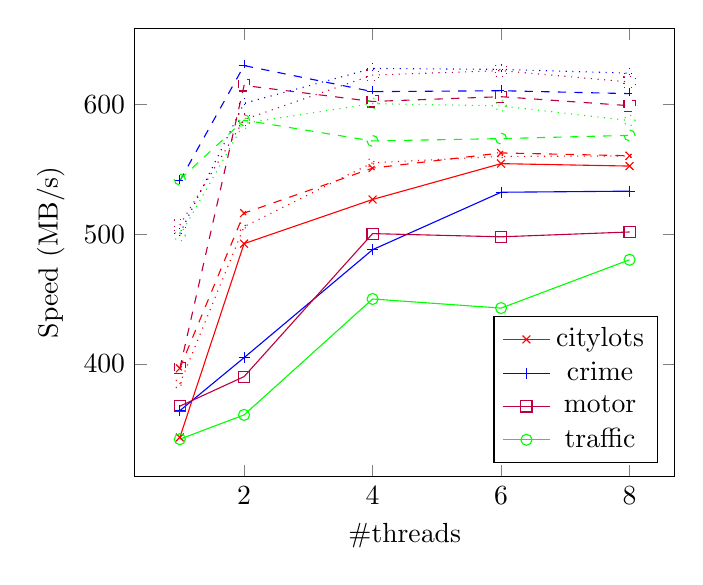
\begin{tikzpicture}
    	\begin{axis}[
    		xlabel=\#threads,
    		ylabel=Speed (MB/s),
    		legend pos=south east,
    	]
    	% citylots
    	\addplot[color=red,mark=x] coordinates {
        	(1,343.44) (2,492.75) (4,526.78) (6,554.40) (8,552.52)
        };
        % crime
        \addplot[color=blue,mark=+] coordinates {
        	(1,364.04) (2,404.88) (4,488.07) (6,532.35) (8,533.19)
        };
        % motor
        \addplot[color=purple,mark=square] coordinates {
        	(1,367.51) (2,390.29) (4,500.48) (6,498.01) (8,501.73)
        };
        % traffic
        \addplot[color=green,mark=o] coordinates {
        	(1,342.06) (2,360.79) (4,450.10) (6,443.08) (8,480.33)
        };
        % citylots
    	\addplot[color=red,mark=x,dashed] coordinates {
        	(1,396.67) (2,516.28) (4,550.93) (6,562.65) (8,560.47)
        };
        % crime
        \addplot[color=blue,mark=+,dashed] coordinates {
        	(1,541.13) (2,629.96) (4,609.90) (6,610.60) (8,608.34)
        };
        % motor
        \addplot[color=purple,mark=square,dashed] coordinates {
        	(1,396.67) (2,614.67) (4,602.31) (6,605.99) (8,599.05)
        };
        % traffic
        \addplot[color=green,mark=o,dashed] coordinates {
        	(1,542.16) (2,587.90) (4,571.88) (6,573.69) (8,576.19)
        };
        % citylots
    	\addplot[color=red,mark=x,dotted] coordinates {
        	(1,384.67) (2,505.81) (4,555.07) (6,559.97) (8,560.34)
        };
        % crime
        \addplot[color=blue,mark=+,dotted] coordinates {
        	(1,500.53) (2,600.91) (4,627.78) (6,627.05) (8,624.10)
        };
        % motor
        \addplot[color=purple,mark=square,dotted] coordinates {
        	(1,507.10) (2,588.39) (4,622.65) (6,626.06) (8,617.31)
        };
        % traffic
        \addplot[color=green,mark=o,dotted] coordinates {
        	(1,498.85) (2,585.46) (4,600.67) (6,598.86) (8,587.60)
        };
    \legend{citylots, crime, motor, traffic}
	\end{axis}
\end{tikzpicture}
    \caption{Speed up with different number of threads for FSM parser. Solid line: no dedicated string parsing threads. Dashed line: 2 dedicated string parsing threads. Dotted line: 4 dedicated string parsing threads. Experiments executed on Intel i5-6200U 2.3GHz CPU (Skylake) with 4 cores.}
    \label{fig:speedup}
\end{figure}

\section{Conclusion}

In conclusion, using multi-threading to optimize JSON parsing is possible and could be useful for large JSON files. The overhead of multi-threading makes it hard to compete with single thread based parsing algorithm on small cases. The SIMD optimization, on the other hand, can accelerate the parsing under different scenarios which makes its performance more robust. There is still some room for further optimization. With our multi-threading optimization, the second stage of parsing is not the bottleneck any more and the first stage currently is not optimized with multi-threading. It might be not trivial to develop a multi-thread version for that as the parsing in stage 1 always depends on limited mask results from previous step. We expect performance could be improved further on top of that.

\section{Division of Work}

Da reimplemented stage 1 as described in \texttt{simdjson} (extracting structural characters using SIMD). Zecong and Da collaboratively worked on the re-implementation of the tape-based storage and FSM parser in stage 2. Zecong implemented the shift-reduce parser and multi-threading for FSM parser. Both students performed benchmark testing.

\bibliography{main}
\bibliographystyle{plain}

\end{document}
